\documentclass[letterpaper,12pt]{article}

%\usepackage{ucs}
%\usepackage[utf8x]{inputenc}
\usepackage{amsmath}
\usepackage{amsfonts}
\usepackage{amssymb}
\usepackage{graphicx}
%\usepackage[canadian]{babel}
\usepackage[margin=1in]{geometry}
\usepackage{multicol}
\newcommand{\R}{\mathbb{R}}
\renewcommand{\i}{\mathbf{i}}
\renewcommand{\j}{\mathbf{j}}
\renewcommand{\k}{\mathbf{k}}
\newcommand{\pd}[2]{\dfrac{\partial #1}{\partial #2}}
\newcommand{\di}{\displaystyle}

\title{Solutions to Quiz 10 Practice Problems\\Math 2580\\Spring 2016}
\author{Sean Fitzpatrick}
\date{February 23rd, 2016}

\begin{document}
 \maketitle
\begin{enumerate}
 \item Find the following antiderivatives:
\begin{enumerate}
 \item $\di \int e^{3x}\,dx = \frac{1}{3}e^{3x}+C$ (letting $u=3x$)
 \item $\di \int \cos(x)\,dx = \sin(x)+C$ (immediate)
 \item $\di \int \frac{2x}{1+x^2}\,dx = \ln(1+x^2)+C$ (letting $u=1+x^2$)
 \item $\di \int x\sin(x)\,dx = -x\cos(x)+\sin(x)+C $ (by parts)
 \item $\di \int \sin^2(x)\,dx = \int \frac{1}{2}(1-\cos(2x))\,dx = \frac{x}{2}-\frac{1}{4}\sin(2x)+C$
 \item $\di \int \frac{1}{\sqrt{4-x^2}}\,dx = \sin^{-1}\left(\frac{x}{2}\right)+C$
\end{enumerate}

 \item Sketch the following rectangles in $\R^2$:\label{a}
\begin{multicols}{2}
\begin{enumerate}
 \item $[-1,2]\times [0,2]$

\begin{center}
 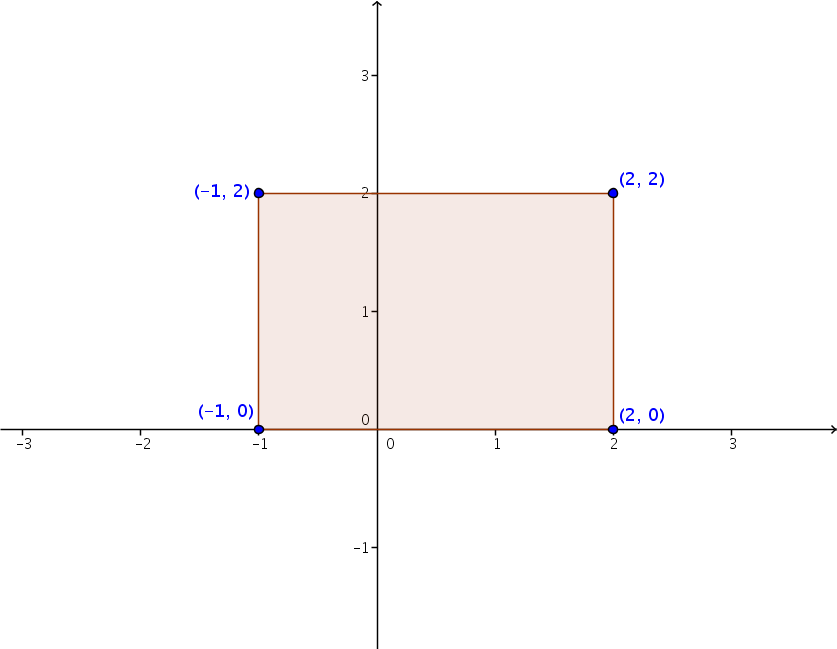
\includegraphics[width=2.5in]{Q10-2a.png}
\end{center}



 \item $[1,4]\times [-1,1]$

\begin{center}
 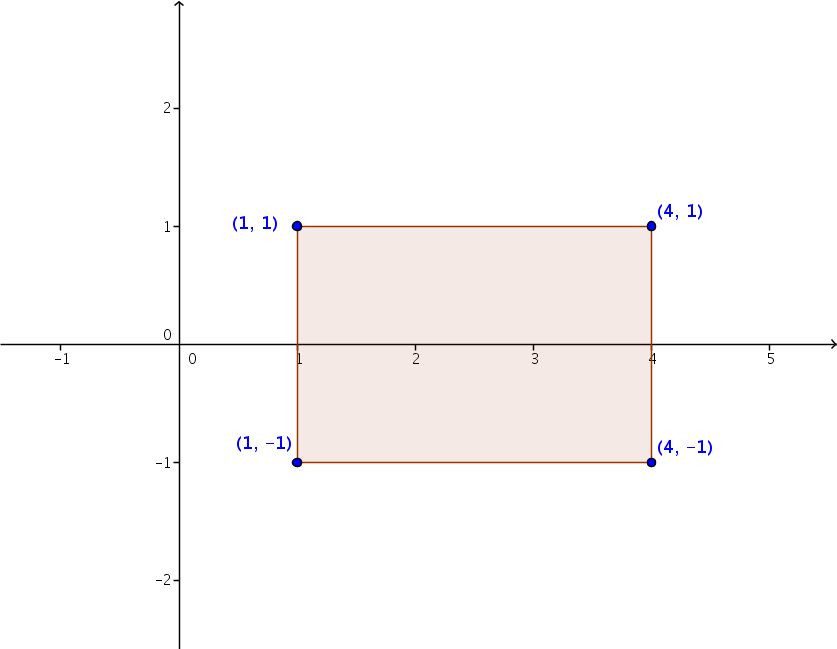
\includegraphics[width=2.5in]{Q10-2b.png}
\end{center}

\end{enumerate}
\end{multicols}
 \item For each of the rectangles from Problem \ref{a}, determine uniform partitions $x_0<x_1<x_2<x_3$ of the $x$-interval into three sub-intervals and $y_0<y_1<y_2$ of the $y$-interval into two sub-intervals. Use these partitions to divide the given rectangle into six sub-rectangles $R_{ij}$, with $1\leq i\leq 3$ and $1\leq j\leq 2$. 

\begin{enumerate}
 \item We let $x_0=-1, x_1=0, x_2=1, x_3=2$, and $y_0=0, y_1=1, y_2=2$. The corresponding rectangles are $R_{1,1}=[-1,0]\times [0,1], R_{1,2} = [-1,0]\times [1,2], R_{2,1} = [0,1]\times [0,1], R_{2,2} = [0,1]\times [1,2], R_{3,1} = [1,2]\times [0,1], R_{3,2} = [1,2]\times [1,2].$
\begin{center}
 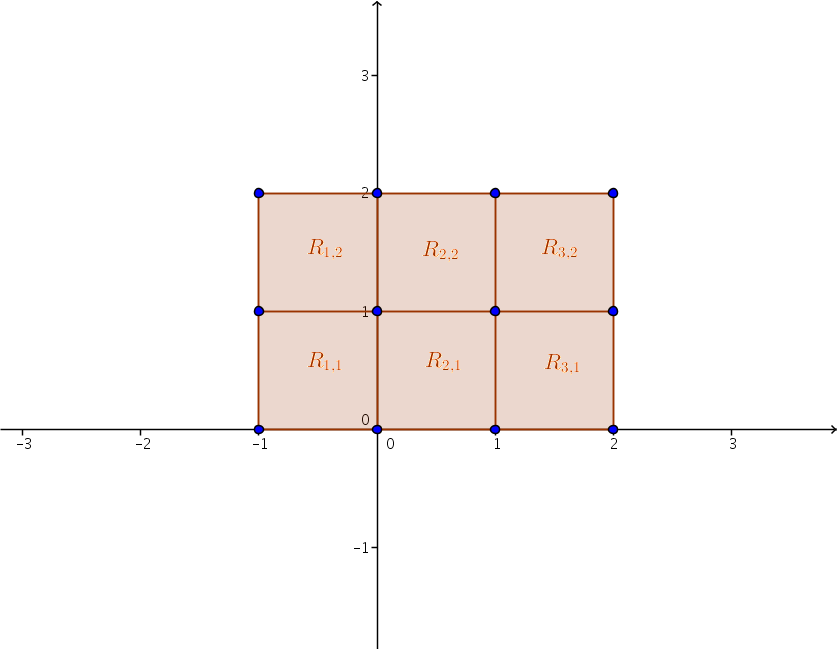
\includegraphics[width=3.5in]{Q10-3a.png}
\end{center}
 \item We let $x_0=1, x_1=2, x_2=3, x_3=4$ and $y_0=-1, y_1 = 0, y_1 = 1$. The corresponding rectangles are $R_{1,1}=[1,2]\times [-1,0], R_{1,2} = [1,2]\times [0,1], R_{2,1} = [2,3]\times [-1,0], R_{2,2} = [2,3]\times [-1,0], R_{3,1} = [3,4]\times [-1,0], R_{3,3} = [3,4]\times [0,1].$
\begin{center}
 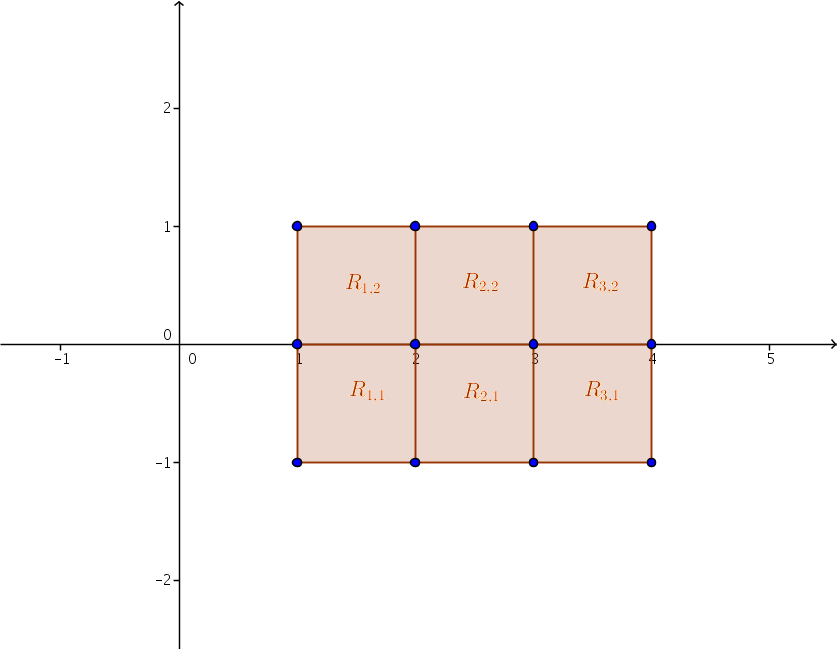
\includegraphics[width=3.5in]{Q10-3b.png}
\end{center}
\end{enumerate}
\pagebreak
 \item Sketch each of the subsets of $\R^2$ below and express them as both a Type 1 region and a Type 2 region:
\begin{enumerate}
 \item The region bounded by the coordinate axes and the line $x+y=1$.

\begin{center}
 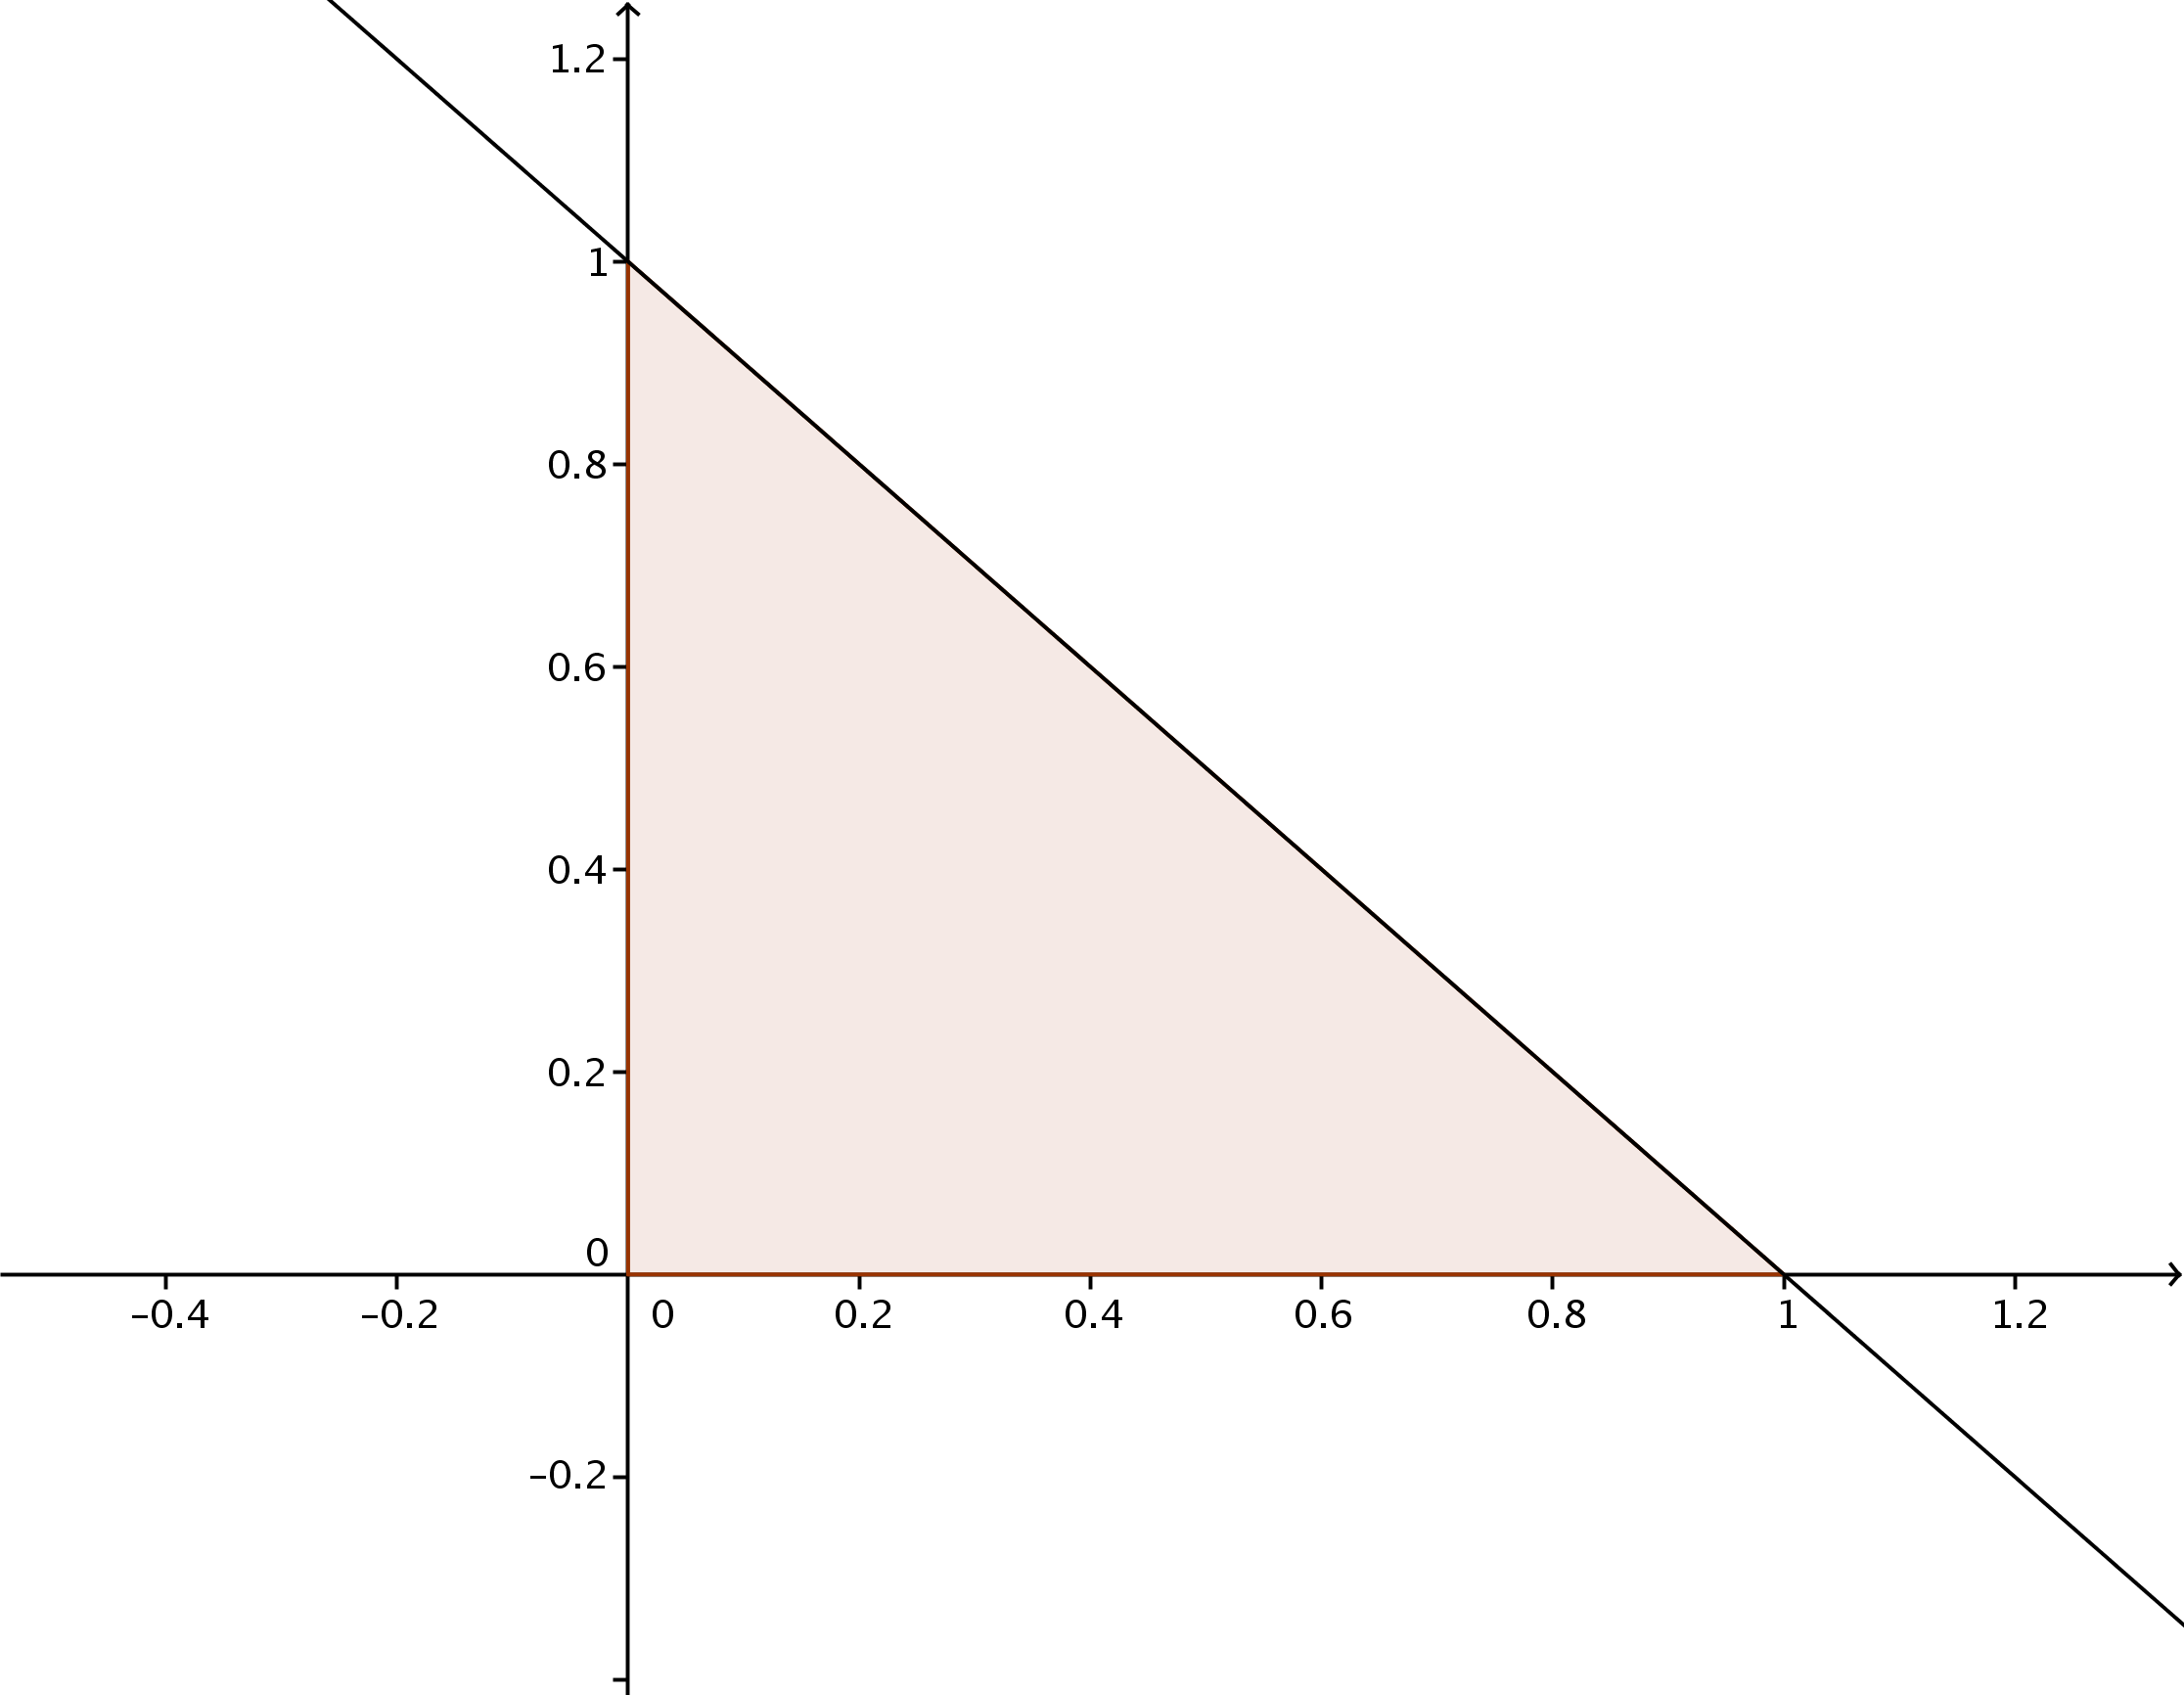
\includegraphics[width=3.5in]{Q10-4a.png}
\end{center}

As a Type 1 region, it is given by the inequalities $0\leq y\leq 1-x$; $0\leq x\leq 1$. As a Type 2 region, it is given by the inequalities $0\leq x\leq 1-y$; $0\leq y\leq 1$.
 \item The region bounded by the curves $y=\sqrt{x}$, $y=0$, and $x=4$.

\begin{center}
 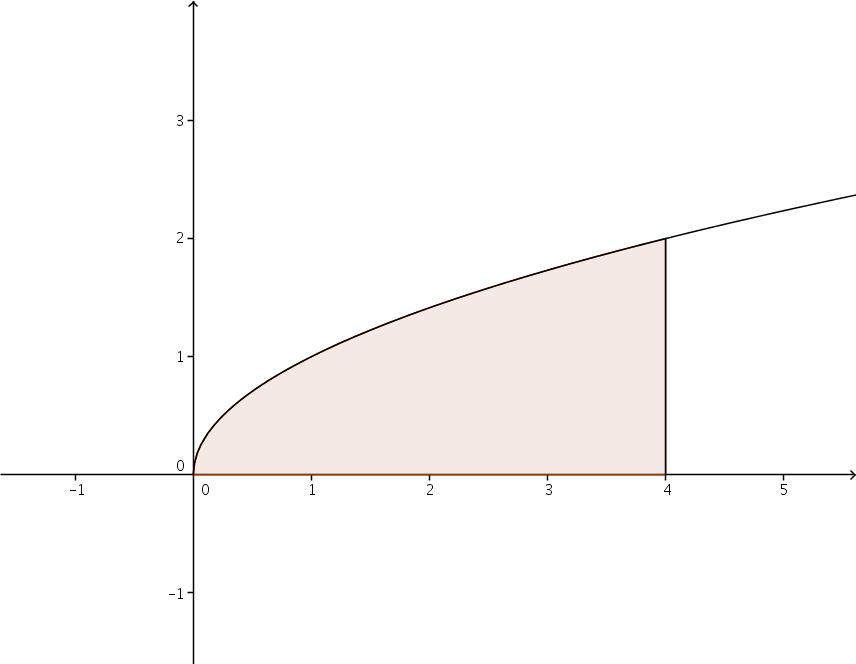
\includegraphics[width=3.5in]{Q10-4b.png}
\end{center}

As a Type 1 region, it is given by $0\leq y\leq \sqrt{x}$; $0\leq x\leq 4$. As a Type 2 region, it is given by $y^2\leq x\leq 4$; $0\leq y\leq 2$.
\end{enumerate}

 \end{enumerate}

\end{document}
 
